\documentclass[12pt, a4paper]{article}
\usepackage[utf8]{inputenc}
\usepackage[margin=1in]{geometry}
\usepackage{graphicx}

\usepackage{tikz}
\usetikzlibrary{shapes,arrows}
\usetikzlibrary{calc}
\usepackage{setspace}
\usepackage{listings}
\usepackage{enumitem}
\usepackage{algorithm}
\usepackage{algpseudocode}
\usepackage{pifont}
\onehalfspacing
\begin{document}
\newpage

\section{ABSTRACT}

\hspace{3cm}
Computer vision is an interdisciplinary field that deals with how computers can be made to gain high-level understanding from digital images or videos. From the perspective of engineering, it seeks to automate tasks that the human visual system can do. It is concerned with modeling and replicating human vision using computer software and hardware.
\par Here we analyze traffic using Computer Vision. Vehicle detection and tracking
applications play an important role for civilian and military applications such as in highway traffic surveillance control management and urban traffic planning. We count the number of 2 wheeler and 4 wheeler vehicles that are passing given a highway video footage using background subtraction. The system uses background subtraction method to detect vehicles. Experimental results show that this method can detect moving vehicles fast and accurately in complex traffic situation.
\vspace{1.5cm}

\section{ACKNOWLEDGEMENT}
\par \vspace{0.25cm} The elation and gratification of this seminar will be incomplete without mentioning all the people who helped me to make it possible, whose gratitude and encouragement were invaluable to me.
\vspace{0.25cm}        
\par I express my sincere gratitude to our guide \textbf{Prof.Guru R} for his valuable words of advice. 
I would like to thank \textbf{Dr.H.C.Vijayalakshmi, Head of Department} for her support and guidance.
\vspace{0.25cm}  
    \par I am also thankful to all the other lecturers and friends without whom this would not have been possible.
\newpage
\tableofcontents
\newpage
\begin{Large}\section{INTRODUCTION}\end{Large}
\begin{large}\subsection{Computer Vision}\end{large}
\hspace{3cm}
Computer vision is concerned with modeling and replicating human vision using computer software and hardware. Formally if we define computer vision then its definition would be that computer vision is a discipline that studies how to reconstruct, interrupt and understand a 3d scene from its 2d images in terms of the properties of the structure present in scene.
\par Computer vision is divided into three basic categories that are as following:
\begin{itemize}
\item Low-level vision: includes process image for feature extraction.
\item Intermediate-level vision: includes object recognition and 3D scene Interpretation
\item High-level vision: includes conceptual description of a scene like activity, intention and behavior.
\end{itemize}
\begin{large}\subsection{Applications of Computer Vision}\end{large}
\hspace{3cm}
\begin{itemize}
\item Robotics : One of the major applications is Localization i.e to determine robot location automatically. It is also used in navigation and obstacle avoidance. Human Robot Interaction (HRI) - Intelligent robotics to interact with and serve people is still an area under research.

\item Medicine : For Classification and detection (e.g. lesion or cells classification and tumor detection). It is excessively used in 3D human organ reconstruction (MRI or ultrasound). Vision-guided robotics surgery is employed in some parts of the world.

\item Industrial Automation : It is widely used for Industrial inspection (defect detection). Other applications are bar code and package label reading and Document understanding (e.g. OCR).

\item Security Application : Used majorly in Biometrics (iris, finger print, face recognition).

\item Transportation Application : Used in Autonomous vehicles and in traffic surveillance.

\end{itemize}

\begin{large}\subsection{Computer Vision in Traffic Analysis}\end{large}
\hspace{3cm}
The result of the increase in vehicle traffic, many problems have appeared. For example,
traffic accidents, traffic congestion, traffic induced air pollution and so on. Traffic congestion has been a significantly challenging problem. It has widely been realized that increases of preliminary transportation infrastructure, more pavements, and widened road, have not been able to relieve city congestion. As a result, many investigators have paid their attentions on Intelligent Transportation System (ITS), such as predict the traffic flow on the basis of monitoring the activities at traffic intersections for detecting congestion. We process the information and monitor the results as to better understand traffic flow.
\par
Automatic detecting and tracking vehicles in video surveillance data is a very challenging
problem in computer vision with important practical applications, such as traffic analysis and security. Video cameras are a relatively inexpensive surveillance tool. Manually reviewing the large amount of data they generate is often impractical. Thus, algorithms for analyzing video which require little or no human input is a good solution. Video surveillance systems are focused on background modeling, moving vehicle classification and tracking. The increasing availability of video sensors and high performance video processing hardware opens up exciting possibilities for tackling many video understanding problems, among which vehicle tracking and target classification are very important. A vehicle tracking and classification system is described as one that can categorize moving vehicles and further classifies the vehicles into various classes.


\newpage
\begin{Large}\section{OBJECTIVES}\end{Large}
\hspace{3cm}
\begin{itemize}
\item To develop a vision based surveillance system capable of identifying vehicles in the scene.
\item To track the vehicles as they progress along the image sequence.
\item To classify the vehicles as 2 wheelers and 4 wheelers
\item To count the number of vehicles passing.
\end{itemize}

\newpage
\begin{Large}\section{PROPOSED SYSTEM}\end{Large}
\hspace{3cm}The proposed system mainly uses Background subtraction technique for detection of vehicle. The background is created by taking the continuous average of accumulated weight of first few frames and is gray scaled. Then the newly obtained frames are also grayscaled for ease of processing. The foreground is extracted by taking the absolute difference of the new frame and the background. The result is subjected to thresholding and is binarized so that all the white zones are considered as vehicles and the black zones are rejected. This may include some noise which is then removed by using erosion and dilation. Contours are drawn around the white subjects in the newly filtered image and centroids of the contours are stored. The vehicle is tracked using tricky algorithm and it is counted only when the vehicle passes a virtual line.
\par The whole system is implemented in Python 3 using OpenCV module.
\\
\\
\begin{large}\subsection{OpenCV}\end{large}
\hspace{3cm}
Open CV is an open source project. The library is an implementation of
some data structures and algorithms are found useful in Computer Vision.
\par Computer vision is a rapidly growing field, partly as a result of both cheaper and more capable cameras, partly because of affordable processing power, and partly because vision algorithms are starting to mature. Open CV itself has played a role in the growth of computer vision by enabling thousands of people to do more productive work in vision. With its focus on real-time vision, Open CV helps students and professionals efficiently implement projects and jump-start research by providing them with a computer vision and machine learning infrastructure that was previously available only in a few mature research labs.

\newpage
\begin{large}\subsection{Design}\end{large}
The design is shown in the below figure.
\begin{figure}[h!]\includegraphics[width=\linewidth]{design.png}\caption{System Design}\end{figure}


\newpage
\begin{Large}\section{Implementation}\end{Large}
\begin{large}\subsection{Background Registration}\end{large}
\hspace{3cm}
Background registration is the most important job in vision based surveillance systems. The background is created by taking the continuous average of accumulated weight of first few frames and is gray scaled. The algorithm is as follows
\\
\begin{algorithm}
\caption{Background Registration algorithm}
\label{CHalgorithm}
\begin{algorithmic}[1]
\Procedure{get background}{alpha , no of frames}
\\result = empty frame
\For{1 : no of frames }
\State Retrieve new frame from the camera
\State result = ( 1 - alpha )result + ( alpha )new frame
\EndFor
\\result = grayscale(result)
\\return result
\EndProcedure
\end{algorithmic}
\end{algorithm}

\begin{large}\subsection{Frame Extraction and Grayscaling}\end{large}
\hspace{3cm}
The video to be processed in nothing but a series of images or frames. Each frame is accessed individually and processed. OpenCV provides us with methods to extract individual frames with ease. Before processing the frame, we convert it to grayscale.
\\
\begin{large}\subsubsection{Why should we grayscale ?}\end{large}
\hspace{3cm}
Converting to gray scale is not necessary for image processing, but is usually done for a few reasons:
\begin{itemize}
\item Simplicity - Many image processing operations work on a plane of image data (e.g., a single color channel) at a time. So if you have an RGBA image you might need to apply the operation on each of the four image planes and then combine the results. Gray scale images only contain one image plane (containing the gray scale intensity values).
\item Data reduction - Suppose you have a RGBA image (red-green-blue-alpha). If you converted this image to gray scale you would only need to process 1/4 of the data compared to the color image. For many image processing applications, especially video processing (e.g., real-time object tracking), this data reduction allows the algorithm to run in a reasonable amount of time.
\end{itemize}
However, it's important to understand that while there are many advantages of converting to gray scale, it is not always desirable. When you convert to gray scale you not only reduce the quantity of image data, but you also lose information (e.g., color information). For many image processing applications color is very important, and converting to gray scale can worsen results.
\begin{large}\subsubsection{How do we Grayscale images in OpenCV ?}\end{large}
\hspace{3cm}
Converting image to grayscale is a simple task in OpenCV.It provides a function "cvtColor()" for the same. It uses the following formula.\\
\[ Y = 0.299 R + 0.587 G + 0.114 B \]
\begin{large}\subsection{Background Subtraction}\end{large}
\hspace{3cm}
Background subtraction is done to obtain the objects in the foreground i.e for detection of vehicles. Here we take the absolute difference between the registered background and the current frame. Since both the images are grayscaled it is very easy to calculate the difference and for further processing. OpenCV provides us with a function called ``absdiff()" to carry out the process. The figure below clearly shows the background subtraction process. 
\begin{figure}[h!]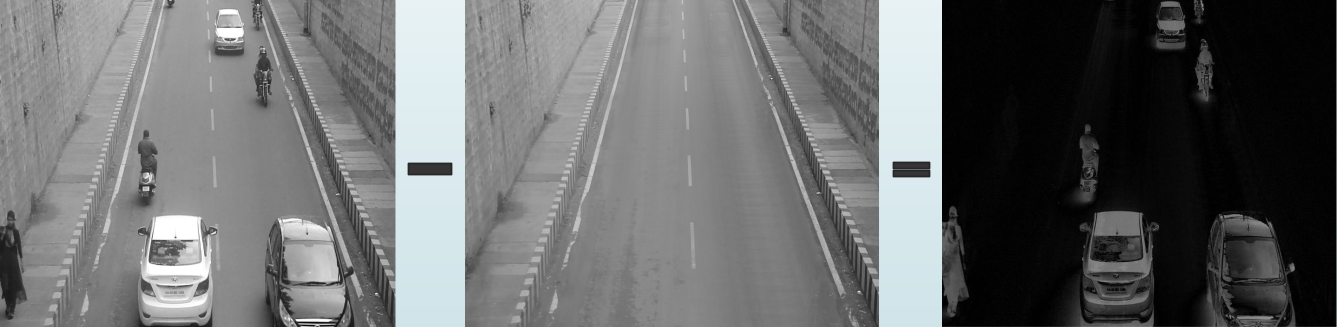
\includegraphics[width=\linewidth]{subtraction.png}\caption{Background Subtraction}\end{figure}
\begin{large}\subsection{Thresholding}\end{large}
\hspace{3cm}
The next step is Binarization. After obtaining the subtracted image, the image has to be segmented into regions containing vehicle and the regions containing non-vehicle. This is decided on the intensity of the region. If the region has an intensity greater than a specified threshold, it is converted to white and the rest is black. OpenCV provides a function ``threshold()" for this purpose. The effect of thresholding can be clearly observed below.
\begin{figure}[h!]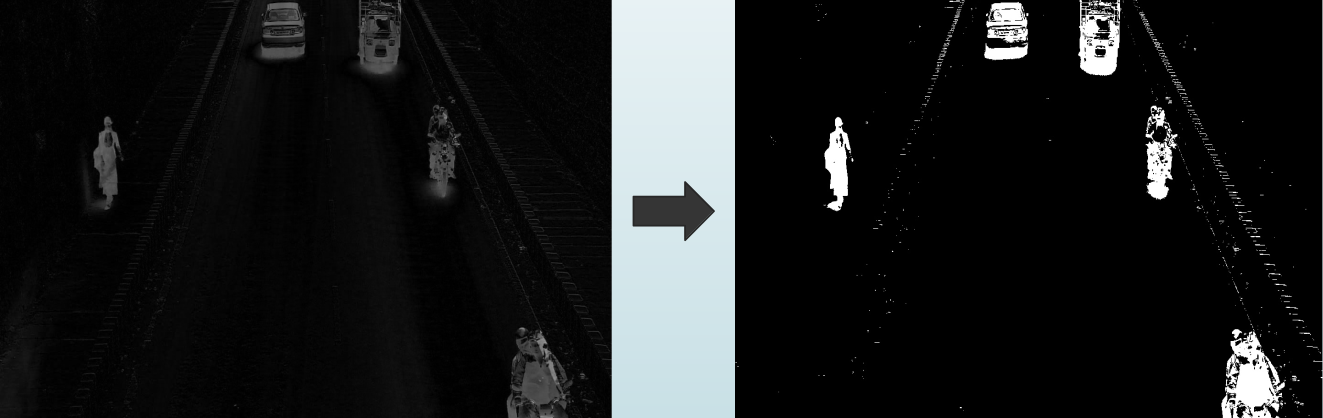
\includegraphics[width=\linewidth]{threshold.png}\caption{Thresholding}\end{figure}
\begin{large}\subsection{Noise Reduction}\end{large}
\hspace{3cm}
It can be observed that the thresholded image has a lot of noise which need to be removed. For this we employ the following 2 techniques.
\\
\begin{large}\subsubsection{Erosion}\end{large}
\hspace{3cm}
Erosion is one of two fundamental operations in morphological image processing from which all other morphological operations are based. The erosion operator takes two pieces of data as inputs. The first is the image which is to be eroded. The second is a (usually small) set of coordinate points known as a structuring element (also known as a kernel). It is this structuring element that determines the precise effect of the erosion on the input image.The mathematical definition of erosion for binary images is as follows:
\begin{itemize}
\item Suppose that X is the set of Euclidean coordinates corresponding to the input binary image, and that K is the set of coordinates for the structuring element.
\item Let Kx denote the translation of K so that its origin is at x.
\item Then the erosion of X by K is simply the set of all points x such that Kx is a subset of X.
\end{itemize}
To compute the erosion of a binary input image by this structuring element, we consider each of the foreground pixels in the input image in turn. For each foreground pixel (which we will call the input pixel) we superimpose the structuring element on top of the input image so that the origin of the structuring element coincides with the input pixel coordinates. If for every pixel in the structuring element, the corresponding pixel in the image underneath is a foreground pixel, then the input pixel is left as it is. If any of the corresponding pixels in the image are background, however, the input pixel is also set to background value. OpenCV provides ``erode()" function for this process. The below figure shows how noise is removed by erosion.
\begin{figure}[h!]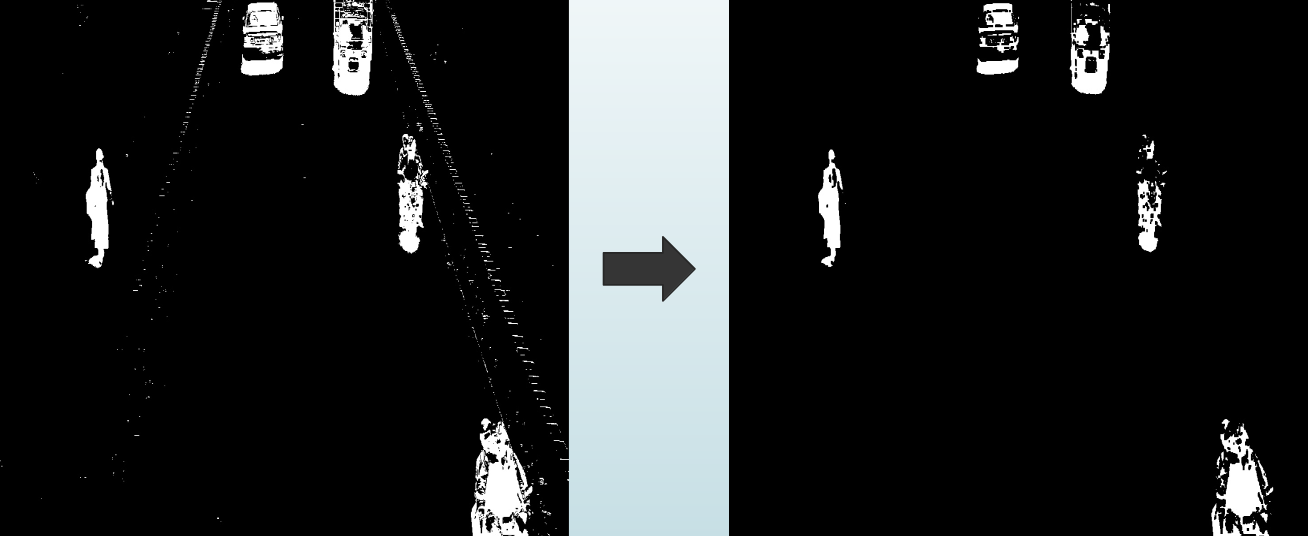
\includegraphics[width=\linewidth]{erosion.png}\caption{Erosion}\end{figure}
\begin{large}\subsubsection{Dilation}\end{large}
\hspace{3cm}
Dilation is one of the two basic operators in the area of mathematical morphology, the other being erosion.The dilation operator takes two pieces of data as inputs. The first is the image which is to be dilated. The second is a (usually small) set of coordinate points known as a structuring element (also known as a kernel). It is this structuring element that determines the precise effect of the dilation on the input image.The mathematical definition of dilation for binary images is as follows:
\begin{itemize}
\item Suppose that X is the set of Euclidean coordinates corresponding to the input binary image, and that K is the set of coordinates for the structuring element.
\item Let Kx denote the translation of K so that its origin is at x.
\item Then the dilation of X by K is simply the set of all points x such that the intersection of Kx with X is non-empty.
\end{itemize}
To compute the dilation of a binary input image by this structuring element, we consider each of the background pixels in the input image in turn. For each background pixel (which we will call the input pixel) we superimpose the structuring element on top of the input image so that the origin of the structuring element coincides with the input pixel position. If at least one pixel in the structuring element coincides with a foreground pixel in the image underneath, then the input pixel is set to the foreground value. If all the corresponding pixels in the image are background, however, the input pixel is left at the background value.OpenCV provides ``dilate()" function for this process. The below figure shows how the holes in the objects are filled and lost data due to erosion is recovered back by dilation.
\begin{figure}[h!]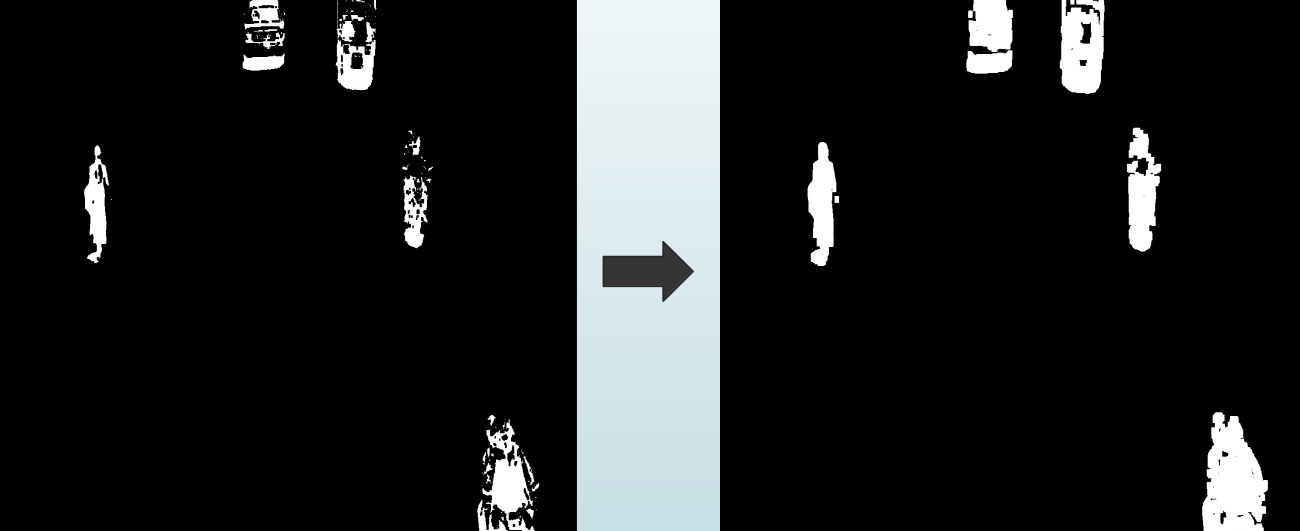
\includegraphics[width=\linewidth]{dilation.png}\caption{Dilation}\end{figure}
\begin{large}\subsection{Vehicle Detection}\end{large}
\hspace{3cm}
After the noise removal , the frame is ready for vehicle detection. All the regions that are white(or 1) are considered as vehicles and the rest as non-vehicles. We take contours of all the vehicle regions , calculate the smallest rectangle that will fit the contour and draw bounding boxes. OpenCV provides the functions ``findContours()" which finds the contours for all the white regions in the frame. Another function ``boundingRect()" calculates the coordinates and size of smallest rectangle to fit the contour. These rectangles are drwn on the frame. The following figure shows drawing bounding boxes around the vehicles. After this the vehicles are tracked using the centroids of these bounding boxes. The below figure shows drawing of these bounding boxes and centroids.\\
\begin{figure}[h!]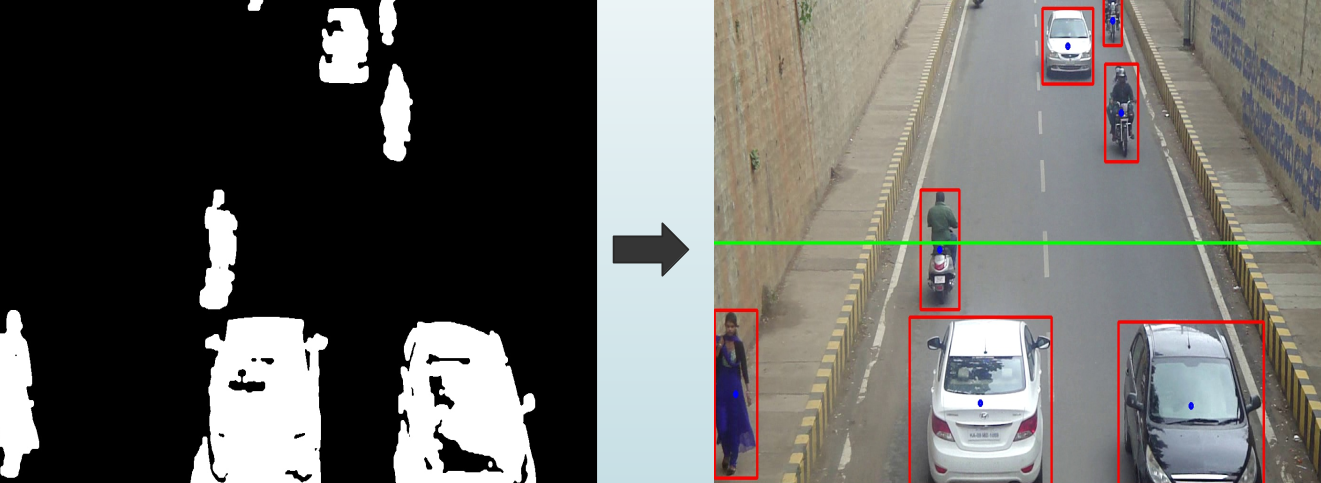
\includegraphics[width=\linewidth]{bounding.png}\caption{Draw Bounding Boxes}\end{figure}
\begin{large}\subsection{Vehicle Counting and Classification}\end{large}
\begin{large}\subsubsection{Counting}\end{large}
\hspace{3cm}
We employ a small tricky algorithm for counting.A vehicle is counted only when the centroid of its bounding box passes through the virtual line.To make sure that a vehicle is counted only once , we also store the centroids of previous frame and use them comparison.A vehicle will be counted if its centroid of current frame has crossed the virtual line and the centroid of previous frame has not crossed the line.The algorithm is as follows: 
\\
\begin{algorithm}[H]
\caption{Check if the vehicle crossed the line}
\label{algo}
\begin{algorithmic}[1]
\Procedure{Check crossing}{count , old centroids , current centroids }
\For{each centroid c1 in current centroids }
\State c2 = position of centroid in previous frame
\If{c1 is above the virtual line and c2 is below the virtual line}
\State count = count + 1
\EndIf
\If{c1 is below the virtual line and c2 is above the virtual line}
\State count = count + 1
\EndIf
\EndFor
\\return count
\EndProcedure
\end{algorithmic}
\end{algorithm}
\begin{large}\subsubsection{Classification}\end{large}
\hspace{3cm}
As soon as the vehicle crosses the line , the next job is classification of vehicles is an easy task. Here we take into account the area under the contours. If the area of the boxes is greater than a specified threshold , it is counted as a 4 wheeler else a 2 wheeler. OpenCV in this regard provides a function ``contourArea()" to calculate area of the contours which helps in classification.
\\
\\
\begin{large}\subsection{Results and Limitations}\end{large}
\hspace{3cm}
We observe the following results
\begin{itemize}
\item With all the false positives considered , the system achieved an accuracy of 90%.
\item The system will easily work in real time with a continuous video stream input of traffic.
\item The system would not work in the night because of the inability of the system to separate background and foreground in low light.
\item Two vehicles moving close to each other are considered as a single object.
\item Occlusion is a another issue. Occluded vehicles are not counted.
\item The system cannot differentiate between vehicles and humans walking down the lane.
\item The camera should be not be moving.
\end{itemize}

\newpage
\section{Conclusion and Future Work}
\hspace{3cm}
Vehicle Detection and Counting is necessary to establish an enriched information platform and improve the quality of intelligent transportation systems. This solution for
Vehicle Detection, Classification and Counting can be used in traffic monitoring, parking area allocation etc.A system has been developed to detect and count dynamic vehicles on highways efficiently. The experimental results show that the accuracy of counting vehicles was 90\% with all the false positives involved.
\par Use of machine learning for detection of vehicles is currently an active area under research. Complex algorithms can be employed in the future which focus on feature based detection of vehicles to handle occlusion and light related issues. Researchers are also working for detection of vehicles using the headlights and the tail lights.

\newpage
\section{REFERENCES}
\begin{itemize}

\item [1] Vehicle detection and tracking techniques: A concise review - Raad Ahmed Hadi1 , Ghazali Sulong and Loay Edwar George
\item [2] Real Time Vehicle Detection and Counting Method for Unsupervised Traffic Video on Highways - Mrs. P.M.Daigavane and Dr. P.R.Bajaj
\item [3] Vehicle detection and counting - Roopashree C , T.R Sateesh kumar



\end{itemize}

\end{document}